%%%%%%%%%%%%%%%%%%%%%%%%%%%%%%%%%%%%%%%%%%%%%%%%%%%%%%%%%%%%%%%%%%%%%%%%%%%%%
\chapter{Sequence-to-Sequence Task-Oriented Dialogue Modeling}
\label{06:chap:lm-tod}
%%%%%%%%%%%%%%%%%%%%%%%%%%%%%%%%%%%%%%%%%%%%%%%%%%%%%%%%%%%%%%%%%%%%%%%%%%%%%
Using end-to-end trainable models instead of modular architectures (see Section~\ref{02:sec:basics}) can can potentially offer more flexibility with respect to domain transfer, as only a single module needs to be adapted to new domains or use cases.
In task-oriented dialogue, end-to-end implementations are dominated by sequence-to-sequence architectures based on language models (LM, Section~\ref{relwork:end-to-end}).
The LM-based approaches have taken over the benchmarks\footnote{\url{https://github.com/budzianowski/multiwoz\#trophy-benchmarks}}, demonstrating state-of-the-art performance.

However, these competitive models are fine-tuned on a large in-domain dataset, and domain transfer performance is not evaluated.
In this chapter, we raise the question of how well these models can transfer the obtained skill of leading the dialogue to other domains.
In other words, we want to discover if the models learn useful skills that can be beneficial in other domains or if the demonstrated behavior merely reproduces the patterns seen in the training portion of the data.
We hypothesize that pre-training of these models can help to improve the performance.
To confirm this hypothesis, we first describe our approach to end-to-end modeling with the GPT-2-based model \cite{kulhanek-etal-2021-augpt} in Section~\ref{06:augpt}.
We then describe our newly assembled and unified multi-domain dataset, designed for domain transfer experiments in Section~\ref{06:sec:diaser} and detail our experimental results with AuGPT on this data in Section~\ref{06:expe}.

The work presented in this chapter was published at the LREC conference and covered by~\citet{hudecek-etal-2022-unifying}
\footnote{This was a joint effort in which the author of this thesis focused on the data processing pipelines and AuGPT model training.}.
For modeling, we use the AuGPT model \cite{kulhanek-etal-2021-augpt} to the development of which we contributed\footnote{The author of this thesis contributed to the model design and data preparation for the training}.
The published experiments in \citet{hudecek-etal-2022-unifying} are further extended to determine if the model can learn from smaller training sets (\ref{06:seed}).
We released the code for data preparation on GitHub\footnote{\url{https://github.com/ufal/diaser}}.

\section{AuGPT Model Description}
\label{06:augpt}
We choose the AuGPT model introduced by \citet{kulhanek-etal-2021-augpt}.
The architecture utilizes the GPT-2 model~\cite{radford2019language} for both belief state prediction and response generation, following the two-step method described in Section~\ref{background:2stage-lm-modeling}.
GPT-2 is a pre-trained language model based on a Transformer decoder.
Therefore, it is suitable for modeling sequences in natural language.
When evaluated with automatic measures, the model performs well, and it showed promising behavior in human-judged interactive evaluation during the DSTC 9 \citep{gunasekara2020overview} challenge. 
AuGPT directly builds on the \emph{small} version of the model, resulting in a 124M parameter model.
Additionally, AuGPT introduces multiple training improvements.
Instead of solely using cross-entropy loss for language modeling, AuGPT uses an additional training objective for state corruption detection.
During training, the model is randomly presented with corrupted versions of the belief state~\citep{peng2021soloist}.
For corruption, portions of the belief state are replaced with random values.
Several strategies can be used to create the corrupted versions; AuGPT corrupts half of the samples by randomly applying one or more of the following modifications:
\begin{itemize}
    \item Replace the belief state $b$ with another belief state, sampled uniformly randomly from the training data.
    \item Replace the delexicalized response with a different randomly chosen one. If this change is combined with the first one, the delexicalized response and the belief state are taken from the same random sample.
    \item A different valid value is uniformly sampled for each slot in the belief state. In this case, the domain names and order are unchanged (i.e., the active domain is the same).
\end{itemize}
The model learns to predict if the presented belief state corresponds to the respective context in the training example.
This modification aims to improve the robustness of the belief state prediction.
Since GPT can work with any natural language sentences, applying this model to our dialogue datasets is straightforward.

\section{Diaser corpus introduction}
\label{06:sec:diaser}
Motivated by the questions raised in this chapter, we created a collection of several well-established task-oriented dialogue datasets spanning several domains to yield one larger multi-domain corpus which we call \emph{Diaser}.
Specifically, we used: \textbf{MultiWOZ 2.2} (MultiWOZ), \textbf{Schema-guided dialogue} (SGD), \textbf{DSTC2} (DSTC) and \textbf{CamRest676} (CamRest).
For more details about the aforementioned datasets, please refer to Section~\ref{02:sec:input-data-desc}.
The merging process yields a dataset with over 37,000 dialogues, comprising more than 660,000 turns.

\subsection{Theoretical motivation}
We aim to cover as many domains as possible in a unified corpus.
Our source dataset choice is thus mainly based on the level of annotation available -- all source datasets include semantic annotation on the turn level and explicit database interaction. 
Despite the dataset similarities, important differences need to be resolved.

The main task when merging datasets is to unify the different domain-specific ontologies, i.e., the different sets of concepts included in the dialogue acts.
More precisely, the unified dataset ontology contains all the possible domains with corresponding slots and associated value sets.
We cannot consider the slots independently from the domain they belong to.
Indeed, a slot that represents the \textit{price range} will not have the same range of values when relating to a restaurant or a flight ticket.
We identified two main problems related to this issue:
\begin{enumerate}
    \item \textbf{Name reference ambiguities}
    We must design the final ontology so that different slot names refer to different concepts (with due precaution for label choice) and merge different slot names associated with the same value set under a single label.
    For example, in MultiWOZ, there are two different slot names \textit{day} and \textit{book-day} for the same value set (weekdays) and usage contexts.
    But in SGD, these slot names may be misleading since we can find a slot named \textit{start-day} and another called \textit{day}; the former refers to a calendar date while the latter refers to a weekday.
    
    \item \textbf{Absence of ontology/database} When the SGD dataset was collected, the authors used API calls instead of a database lookup.
    They also didn't provide an overall ontology.
    Therefore, no database-related metadata was released with the corpus, forcing us to create an ontology and a database for the data based on values occurring in the conversations.
\end{enumerate}

\subsection{Details of the merging approach}
\begin{table}[tp]
    \centering\footnotesize
    \begin{tabular}{l@{\hspace{0.8em}}r@{\hspace{0.3em}}r@{\hspace{0.3em}}r@{\hspace{0.3em}}r@{\hspace{2em}}r}
        \toprule
        \textbf{Data}         & \textbf{SGD} & \textbf{MultiWOZ} & \textbf{DSTC} & \textbf{CamRest} & \textbf{Total} \\ \midrule
        \textbf{Domains}        & 18        &    7        &      1        &      1      &    19$^{\ast}$ \\
        \textbf{Slots}        & 145       &    29       &     10        &      7      & 166$^{\ast}$ \\
        \textbf{Dialogues$^{\ast\ast}$}       & 22.8    & 10.4     &    3.2     &      0.7   & 37.1\\
        \textbf{Turns$^{\ast\ast}$}        & 463.3   & 143.0     &    51.0  &     5.5   & 662.8\\
        \textbf{Turns/Dial.}   & 20.30     & 13.71       &   15.77        &     8.12    & 17.83 \\
        \textbf{Avg. utt. length} & 9.86      &  13.23      &   8.47        &  10.71       & 10.49 \\
        \textbf{Unique Words}$^{\ast\ast}$ & 32.3 & 23.2 & 1.3 & 1.7 & 49.9 \\
        \textbf{Shannon ent.} & 8.96 & 8.54 & 7.04 & 7.69 & 9.01 \\
        \textbf{Cond. ent.} & 4.76 & 4.41 & 2.14 & 2.95 & 4.83 \\

     \bottomrule
    \end{tabular}
    \caption{Composition of our dataset, with basic statistics, overall and for individual sources (number of domains and slots, total numbers of dialogues and turns, average number of turns per dialogue, and average utterance length in terms of words. $^{\ast}$ is not a sum due to ontology merging. $^{\ast\ast}$ in thousands.}
    \label{06:tab:final_data_stats}
\end{table}
Here, we present details on how we merged the data into a common format, including handling different ontologies.
Quantitative statistics of the final dataset are shown in Table~\ref{06:tab:final_data_stats}.
Full technical documentation can be found in the data repository.\footnote{\url{https://github.com/ufal/diaser}}
Here we list an overview of all the required merging steps:

\paragraph{Matching belief representations.} In DSTC and CamRest, belief state annotations are extracted from the user and the system utterance.
In contrast, in the MultiWOZ and SGD datasets, the belief state is only extracted from the user utterance.
We had to filter automatically the annotations from DSTC and CamRest until they matched the MultiWOZ belief state representation. 
    
\paragraph{Adding meta features} from the original datasets. DSTC2, CamRest, and MultiWOZ contain the \emph{goal} of the dialogue (also called task) as a dialogue act with the constraints (e.g. expensive restaurant south) and the information the user needs to obtain from the system (e.g. phone number and address). They also contain a short text summarizing this goal for crowd workers. We include both versions of the task description with each dialogue.
    
\paragraph{Unifying annotation structure.} The final dataset structure is similar to the structure of SGD and MultiWOZ 2.2. We create a \textit{Turn} object that contains either the user utterance and dialogue acts or the system utterance.
Two consecutive entries for the user and system share the same turn number -- we consider a \textit{Turn} as an exchange between the user and the system (i.e. a pair or utterances). 

\paragraph{Ontology unification.}   
One of the most difficult parts of this work was unifying the ontologies of each original dataset because they were not built on the same dimensions.
This concerns slot, domain, and intent names.

After indexing all annotations from the different datasets, we merged them manually using MultiWOZ as a golden reference to create the mapping.
We always check the meaning in context and match slots/intents with the same semantics.

% In addition to unifying the naming, we also needed to address that the ontologies distinguish between two kinds of slots: informable and requestable (see Section\ref{02:ds-background}).We use this distinction to also assign slots in the other two datasets into one of these two groups.

\paragraph{Slot co-reference}
Some source corpora (MultiWOZ and SGD) include co-reference between slots.
For example, \textit{start-time} can take the value “sooner than that” or the slot \emph{hotel-name} can take the value “event you mentioned earlier”.
This is a problem if we assume a self-contained ontology that captures all the possible values from the corpus.
However, as these co-references are impossible to include in the ontology easily, we leave these values unchanged and the slot co-references are carried over to the unified data.

\begin{table}[tp]
    \centering\footnotesize
    \begin{tabular}{l>{\hspace{-3mm}}r>{\hspace{-2mm}}rrr>{\hspace{-2mm}}r}
        \toprule
        \bf Intent &
        \textbf{SGD} & 
        \textbf{MultiWOZ} &
        \textbf{DSTC} &
        \textbf{CamRest} &
         \textbf{all}\\ \midrule
        \textbf{inform} & 151,467 & 84,259 & 33,451 & 5,786 & 274,963\\ 
        \textbf{request} & 81,786 & 31,888 & 13,620 & 1,516 & 128,810\\ 
        \textbf{offer} & 67,095 & 4,497 & 23,763 & 0 & 95,355\\ 
        \textbf{bye} & 35,089 & 12,380 & 0 & 0 & 47,469\\ 
        \textbf{else}& 31,030 & 13,779 & 0 & 0 & 44,809 \\ 
        \textbf{select}& 33,820 & 2,834 & 243 & 0 & 36,897\\ 
        \textbf{confirm}& 30,327 & 0 & 5,756 & 0 & 36,083\\
        \textbf{thank}& 23,172 & 9,064 & 0 & 0 & 32,326\\ 
        \textbf{negate}& 132,01 & 4,399 & 4,413 & 0 & 22,023\\ 
        \midrule
        \textbf{total}& 435,957 & 163,100 & 81,346 & 7,312 & 718,645\\
        \bottomrule
    \end{tabular}
    \caption{Most frequent intents in our unified schema, for each source dataset individually and overall (with absolute numbers of occurrences).}
    \label{tab:intents}
\end{table}

\begin{table}[tp]
    \centering\footnotesize
    \begin{tabular}{l>{\hspace{-2mm}}rrrrr}
        \toprule
        \bf Slot &
        \textbf{SGD} & 
        \textbf{MultiWOZ} &
        \textbf{DSTC} &
        \textbf{CamRest} &
         \textbf{all}\\ \midrule
        \textbf{name} & 65,999 & 42,215 & 3,135 & 2 & 111,351\\ 
        \textbf{area} & 8,133 & 48,285 & 37,697 & 4,178 & 98,293 \\ 
        \textbf{date} & 81,600 & 20,872 & 0 & 0 & 102,472\\
        \textbf{price} & 1,950 & 33,084 & 32,267 & 4,032 & 71,333\\
        \textbf{type}& 41,146 & 28,562 & 0 & 0 & 69,708\\
        \textbf{leave}& 32,625 & 26,684 & 0 & 0 & 59,309\\
        \textbf{arrive}& 26,180 & 26,228 & 0 & 0 & 52,408\\
        \textbf{food}& 13,501 & 20,963 & 3,007 & 571 & 38,042\\
        \textbf{book}& 17,618 & 11,723 & 0 & 0 & 29,341\\
        \midrule
        \textbf{total}& 298,752 & 232,388 & 76,106 & 8,783 & 532,257\\
        \bottomrule
    \end{tabular}
    \caption{Most frequent slots in our unified schema, for each source dataset individually and overall (with absolute numbers of occurrences).}
    \label{tab:slots}
\end{table}

\section{Experiments}
\label{06:expe}

In this chapter, we want to explore if sequence-to-sequence LM-based architectures can robustly learn the dialogue modeling capabilities and how well they can transfer them to other domains.
To answer these questions, we conduct a series of experiments to train the model using only a small portion of the training data or even a different dataset with shared characteristics such as a task-oriented approach, regular user-system interaction, etc.

We divide the results into two sections.
First, we describe the performance of the AuGPT model when trained and evaluated on various datasets.
In the second section, we show the results when the model is pre-trained on a certain dataset and then fine-tuned using only a small portion of training data from the target dataset.

We are interested in the overall performance of the models.
Therefore, we measure Joint Goal Accuracy and Slot-F1 and BLEU for response generation (see Section~\ref{02:sec:eval_metrics}).
We do not compute the dialogue success as it is not well-defined on all the sub-datasets.

\subsection{Experimental setup}
\label{06:experiments}
For training, we follow~\citep{kulhanek-etal-2021-augpt} with the training setup --
We use PyTorch framework \cite{pytorch} and run the training for 8 epochs on the MultiWOZ data when all the training examples are used.
The AuGPT model described in Section~\ref{06:augpt} consists of 12 transformer blocks with a model layer size equal to 768, having 124 million parameters in total.
For the state corruption detection task, we use a dropout of 0.1 with label smoothing of 0.1.
We use the AdamW optimizer \cite{DBLP:conf/iclr/LoshchilovH19} and employ mixed-precision training \cite{micikevicius2017mixed}.

For the data, we follow the dataset discussed in Section~\ref{06:sec:diaser}.
We use different subsets for training and testing the model, as described for each experiment individually.

\subsection{Influence of training data on the target performance}
\label{06:training_data}
\begin{table*}[tp]
    \centering \small
    \begin{tabular}{ccc >{\hspace{1em}} ccc >{\hspace{1em}} ccc}
      \toprule
       \multicolumn{3}{c}{training} & \multicolumn{3}{c}{evaluation} & \multicolumn{3}{c}{metrics}\\
       \textbf{DSTC} & \textbf{MW} & \textbf{SGD} & \textbf{DSTC} & \textbf{MW} & \textbf{SGD} & \textbf{Slot F1} & \textbf{JGA} & \textbf{BLEU} \\
       %========================================================
       \midrule
       %========================================================
       % mwoz-mwoz
       {\textcolor{red} \xmark} & {\textcolor{green} \cmark} & {\textcolor{red} \xmark} & {\textcolor{red} \xmark} & {\textcolor{green} \cmark} & {\textcolor{red} \xmark} & 0.89 & 0.53 & 18.61 \\
       % schema-mwoz
       {\textcolor{red} \xmark} & {\textcolor{red} \xmark} & {\textcolor{green} \cmark} & {\textcolor{red} \xmark}  & {\textcolor{green} \cmark} & {\textcolor{red} \xmark} & 0.16 & 0.02 & \pz4.01 \\
       % dsctmwoz-mwoz
       {\textcolor{green} \cmark} & {\textcolor{green} \cmark} & {\textcolor{red} \xmark} & {\textcolor{red} \xmark}  & {\textcolor{green} \cmark} & {\textcolor{red} \xmark} & 0.89 & {0.55} & 19.67 \\
       % dstcschema-mwoz
       {\textcolor{green} \cmark} & {\textcolor{red} \xmark} & {\textcolor{green} \cmark} & {\textcolor{red} \xmark}  & {\textcolor{green} \cmark} & {\textcolor{red} \xmark} & 0.17 & 0.03 & \pz5.68 \\
       % mwozschema-mwoz
       {\textcolor{red} \xmark} & {\textcolor{green} \cmark} & {\textcolor{green} \cmark} & {\textcolor{red} \xmark}  & {\textcolor{green} \cmark} & {\textcolor{red} \xmark} & 0.89 & 0.52 & 19.92 \\
       % all-mwoz
       {\textcolor{green} \cmark} & {\textcolor{green} \cmark} & {\textcolor{green} \cmark} & {\textcolor{red} \xmark}  & {\textcolor{green} \cmark} & {\textcolor{red} \xmark} &  0.90 & 0.54 & 21.09 \\
       %========================================================
       \midrule
       %========================================================
       % mwoz-schema
       {\textcolor{red} \xmark} & {\textcolor{green} \cmark} & {\textcolor{red} \xmark} & {\textcolor{red} \xmark} & {\textcolor{red} \xmark} & {\textcolor{green} \cmark} & 0.04 & 0.01 & \pz5.63 \\
       % schema-schema
       {\textcolor{red} \xmark} & {\textcolor{red} \xmark} & {\textcolor{green} \cmark} & {\textcolor{red} \xmark}  & {\textcolor{red} \xmark} & {\textcolor{green} \cmark} & 0.59 & 0.21 & {28.17} \\
       % dstcmwoz-schema
       {\textcolor{green} \cmark} & {\textcolor{green} \cmark} & {\textcolor{red} \xmark} & {\textcolor{red} \xmark}  & {\textcolor{red} \xmark} & {\textcolor{green} \cmark} & 0.03 & 0.01 & \pz5.51 \\
       % dstcschema-schema
       {\textcolor{green} \cmark} & {\textcolor{red} \xmark} & {\textcolor{green} \cmark} & {\textcolor{red} \xmark}  & {\textcolor{red} \xmark} & {\textcolor{green} \cmark} & 0.58 & 0.21 & 27.96 \\
       % mwozschema-schema
       {\textcolor{red} \xmark} & {\textcolor{green} \cmark} & {\textcolor{green} \cmark} & {\textcolor{red} \xmark}  & {\textcolor{red} \xmark} & {\textcolor{green} \cmark} & 0.63 & 0.23 & 27.54 \\
       % all-schema
       {\textcolor{green} \cmark} & {\textcolor{green} \cmark} & {\textcolor{green} \cmark} & {\textcolor{red} \xmark}  & {\textcolor{red} \xmark} & {\textcolor{green} \cmark} & 0.63 & 0.22 & 27.72 \\
       %========================================================
       \midrule
       %========================================================
       % dstcmwoz-all
       {\textcolor{green} \cmark} & {\textcolor{green} \cmark} & {\textcolor{red} \xmark} & {\textcolor{green} \cmark} & {\textcolor{green} \cmark} & {\textcolor{green} \cmark} & 0.28 & 0.12 & 15.30 \\
       % dstcschema-all
       {\textcolor{green} \cmark} & {\textcolor{red} \xmark} & {\textcolor{green} \cmark} & {\textcolor{green} \cmark} & {\textcolor{green} \cmark} & {\textcolor{green} \cmark} &  0.55 & 0.22 & 27.28 \\
       % mwozschema-all
       {\textcolor{red} \xmark} & {\textcolor{green} \cmark} & {\textcolor{green} \cmark} & {\textcolor{green} \cmark} & {\textcolor{green} \cmark} & {\textcolor{green} \cmark} & 0.65 & 0.25 & 25.13 \\
       % all-all
       {\textcolor{green} \cmark} & {\textcolor{green} \cmark} & {\textcolor{green} \cmark} & {\textcolor{green} \cmark} & {\textcolor{green} \cmark} & {\textcolor{green} \cmark} & 0.70 & 0.28 & \textbf{29.73} \\

      \bottomrule
  \end{tabular}
  \caption{Performance of the AuGPT model trained and evaluated on various subsets of the unified dataset, namely DSTC, MultiWOZ (MW), and SGD. We omit CamRest since the data are very similar to DSTC.}
  \label{06:tab:exp-results-diaser}
\end{table*}

In Table~\ref{06:tab:exp-results-diaser}, we can see a general pattern in the results, suggesting that the model fails to generalize across different datasets when a subset of data we evaluate is not included in the training. A significant drop in performance can be observed across all recorded metrics.
We use  DSTC, MultiWOZ (MW), and SGD. We omit CamRest since the data are very similar to DSTC.

Let us first observe some global properties.
Regarding the $F_1$ slot score and joint goal accuracy, the explanation for the poor model's accuracy can be found in a substantially different distribution of slots across SGD/MultiWOZ datasets and DSTC.
Some slots are present in just one of the datasets, others are mentioned in different contexts or with different frequencies.
Training on MultiWOZ provides us with the highest scores on slot $F_1$ and joint goal accuracy.
Training on both SGD and MultiWOZ brings only a very marginal improvement.
The large difference in performance can also be seen in terms of BLEU, which suggests a vastly different language used in each dataset.

The performance of the model evaluated on MultiWOZ is analogous.
Training the model solely on SGD gives us a model that cannot generalize to MultiWOZ data.
Concatenating the MultiWOZ datasets with SGD/DSTC, or both during training, leads to a little improvement, predominantly in terms of BLEU score.
We get the best results when using all three datasets for training and obtain the model with better generalizing capabilities supported by the BLEU score of 21.09.

The model evaluation on SGD data mostly follows the same pattern. However, in this case, it is quite interesting to observe that training the model on all three datasets is not beneficial, and the performance stagnates, although the training set is much larger.

Finally, if we evaluate all three datasets, it is clear that the best-performing model is obtained when we train it on the full data.
Table \ref{tab:exp-results-diaser} shows that including SGD data is crucial for achieving higher BLEU values while training on MultiWOZ helps the model predict slot values.

\subsection{Domain adaptation with a small in-domain set}
\label{06:seed}
Table~\ref{tab:exp-results-seed} presents results for domain adaptation experiments.
We first train the AuGPT model on the MultiWOZ dataset and then use a small portion of the SGD data to adapt the model to this different dataset.
The results show that although on MultiWOZ helps slightly to improve the final BLEU score, the performance of belief state tracking is not significantly improved, and the results are overall rather negative.

\begin{table*}[tp]
    \centering \small
    \begin{tabular}{cccccc}
      \toprule
       pre-training & fine-tuning & ft-ratio & \textbf{Slot-F1} & \textbf{JGA} & \textbf{BLEU} \\
        \midrule
       -- & SGD & 100\% & 0.59 & 0.21 & 28.17 \\
       -- & SGD & 10\% & 0.47 & 0.15 & 20.13 \\
       MultiWOZ & SGD & 10\% & 0.46 & 0.16 & 19.46 \\
       -- & SGD & 5\% & 0.29 & 0.08 & 14.65 \\
       MultiWOZ & SGD & 5\% & 0.29 & 0.12 & 15.16 \\
       -- & SGD & 1\% & 0.07 & 0.03 & 6.37\\
       MultiWOZ & SGD & 1\% & 0.06 & 0.01 & 8.40 \\
       -- & SGD & 0.5\% & 0.04 & 0.04 & 3.43 \\
       MultiWOZ & SGD & 0.5\% & 0.04 & 0.02 & 5.95 \\
       %========================================================
       \midrule
       %=======================================================
      \bottomrule
  \end{tabular}
  \caption{Performance of the AuGPT model trained and evaluated on various subsets of the unified dataset.}
  \label{tab:exp-results-seed}
\end{table*}


\subsection{Dynamics of Successful and Failed Dialogues}
We also perform a detailed quantitative analysis of errors made by the trained models.
We evaluated the AuGPT model trained on the MultiWOZ data with respect to the dialogue success rates.
We only chose the MultiWOZ data due to the additional annotation available in MultiWOZ.
Specifically, MultiWOZ also has user and system dialogues act annotated, which we use in this analysis.
We consider dialogue success as defined in Section~\ref{02:sec:eval_metrics}.

In Figure~\ref{fig:error_distr}, we provide a histogram of dialogue state tracking errors in successful and failed dialogues.
We further identify four reasons that can cause an error:
\begin{enumerate}
    \item A \emph{domain} is wrongly identified.
    \item An \emph{intent} is detected wrongly.
    \item An \emph{inform} value is captured incorrectly.
    \item A \emph{request} was not answered.
\end{enumerate}
We go turn by turn and identify the errors in the dialogue state predicted by the system compared to the expected state.
``All failed" and ``all success" correspond to failed and successful dialogues.
It is thus an evaluation concerning the dialogue as a whole, unlike the turn-level methods, such as evaluating the system's response generation.
In particular, we show the count of cases where some information is understood wrongly by the system (positive values) or is missing completely (negative values).
We can see that in successful dialogues, the system might make some mistakes at first but can recover eventually.
On the other hand, most dialogue failures are caused by missing information in the second half of the dialogue, which suggests that the recovery is not certain.

We made some observations:
\begin{itemize}
    \item For both successful and unsuccessful dialogues, the first turn concentrates the most errors.
    
    \item Generally speaking, the failed dialogues show much superfluous information in the first five speech turns, especially regarding the user's intent. On the other hand, from approximately the fourth speech turn onwards, there is a lot of missing information, especially at the level of the dialogue domain. If we add the missing information with the superfluous information, the error distribution peaks between turns three and seven of the dialogue. 
\end{itemize}

\begin{figure}[tp]
    \centering  \small
    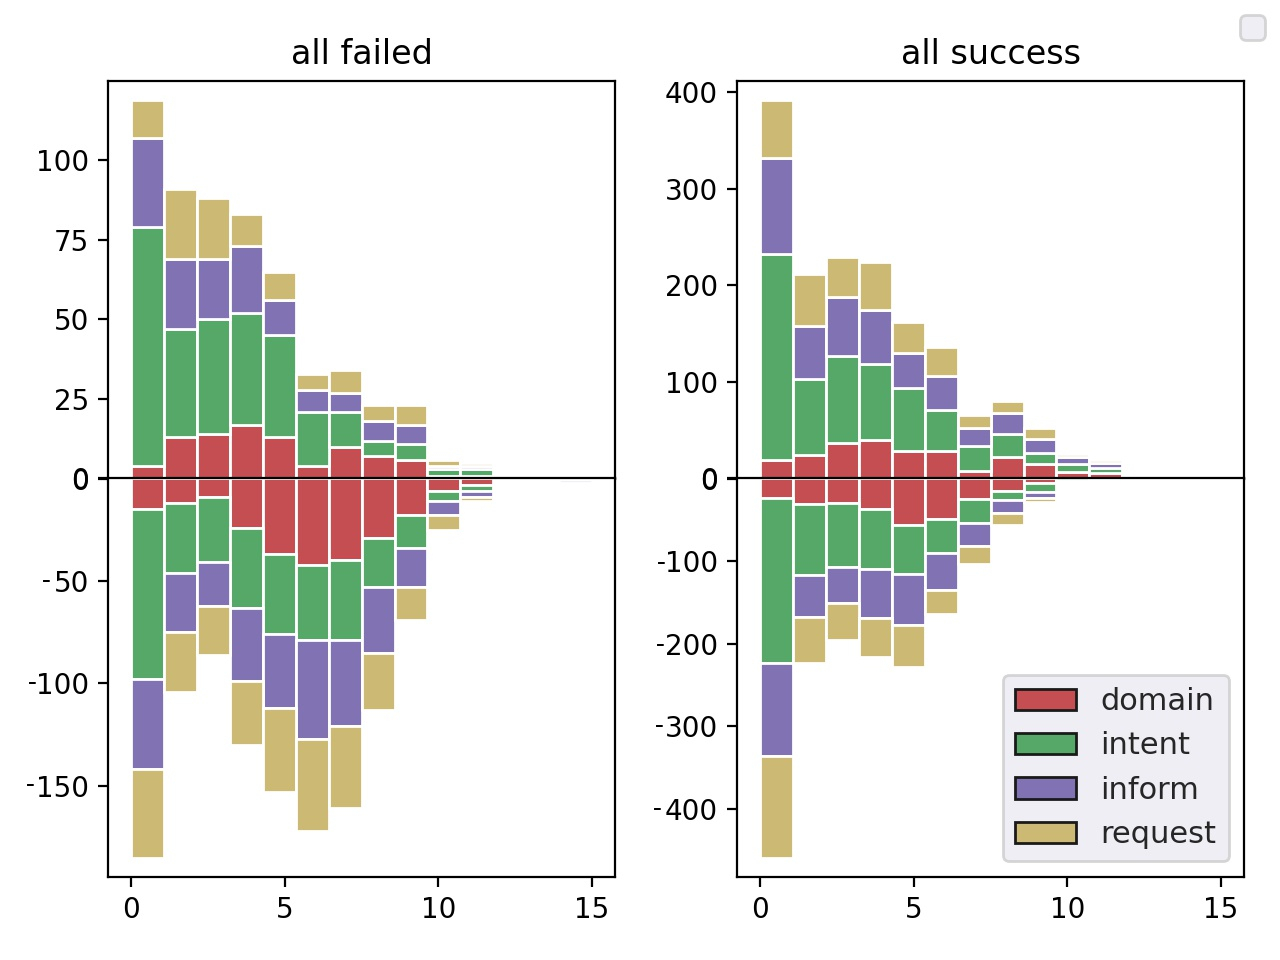
\includegraphics[width=0.49\textwidth]{images/hist-vert-True-gpt.jpg}
    \caption{Distribution and types of dialogue failures that occurred with the GPT2-based model on the MultiWOZ data.
    The horizontal axis corresponds to turn numbers. Positive values represent cases where the information is captured wrongly, while negative values represent cases where particular information is missing.
    The source of error (incorrect domain or intent, missing information, or not providing a request) is depicted as color-coded.}
    \label{fig:error_distr}
\end{figure}



\section{Conclusion}
In this work, we unified a large task-oriented dialogue corpora at both data and annotation levels, which requires a complex process of merging ontologies. 
We showed that additional data from other sources helps train LM-based end-to-end dialogue models when converted to a unified format in specific cases.
However, it is not a general rule.
Although the new dataset is still far from perfect coverage, it is a step towards wider and more authentic data.
We also performed experiments to explore the ability of LM-based systems to adapt to new domains easily with a small number of in-domain examples.
The negative results suggest that using in-domain data for domain adaptation is not straightforward.